\chapter{Anwendungsphase}
\label{chap:workflowTime}

Im Folgenden wird der Prozess vorgestellt, mit dem aus Textsequenzen und einem vorher trainierten Themenmodell die Verläufe der Themen ermittelt werden können. Dazu wird zuerst dargelegt, wie für die neuen Dokumente die Themen ermittelt werden. Dann wird aus den ermittelten Themen für die Dokumente eines Zeitabschnittes ein Graph aufgebaut, dessen Knoten dann mit einem Zentralitätsindex bewertet werden. Anschließend wird veranschaulicht, wie die Verläufe visualisiert werden. Schlussendlich wird vorgestellt, wie die Methode auf ihre Aussage und Richtigkeit überprüft wird.

\section{Frames}

Zuerst wird die Textsequenz in gleich große diskrete Zeitabschnitte unterteilt, Frames genannt. Es ist dabei nicht nötig, dass die Frames disjunkt sind. Es muss jedoch gelten, dass sie eine Sequenz bilden bzw. eindeutig anzuordnen sind. Für ein Korpus $\corpus=(\frame_1,\frame_2,\ldots,\frame_F)$ gilt:
\begin{enumerate}
\item die einzelnen Frames weisen eine Reihenfolge auf. D.h $\frame_1 <_\frame \frame_2 <_\frame \cdots <_\frame \frame_F$ wobei $<_\frame$ die Ordnung auf den Frames darstellt. 
\item die Frames stellen eine komplette Zerlegung des Korpus dar. D.h. $\corpus=\bigcup^F_{i=0}\frame_i$.
\item die Dokumente innerhalb eines Frames müssen wiederum, wie in der Gesamtsequenz, sortiert sein. Für einen Frame $\frame=(\doc_1,\doc_2,\ldots,\doc_f)$ gilt auch, dass $\doctime(\doc_1) \leq \doctime(\doc_2) \leq \cdots \leq \doctime(\doc_f)$. 
\end{enumerate}

\begin{figure}[ht]
\centering
\psset{unit=0.7cm}
\begin{pspicture}(0,-2)(18,4)
\psline(0,0)(0,3)
\psline(0,0)(2,0)
\psline(0,3)(1.5,3)
\psline(2,0)(2,2.5)
\psline(1.5,3)(2,2.5)
\rput(1,1.5){$\doc_1$}

\psline(3,0)(3,3)
\psline(3,0)(5,0)
\psline(3,3)(4.5,3)
\psline(5,0)(5,2.5)
\psline(4.5,3)(5,2.5)
\rput(4,1.5){$\doc_2$}

\psline(6,0)(6,3)
\psline(6,0)(8,0)
\psline(6,3)(7.5,3)
\psline(8,0)(8,2.5)
\psline(7.5,3)(8,2.5)
\rput(7,1.5){$\doc_3$}

\psline(9,0)(9,3)
\psline(9,0)(11,0)
\psline(9,3)(10.5,3)
\psline(11,0)(11,2.5)
\psline(10.5,3)(11,2.5)
\rput(10,1.5){$\doc_4$}

\psline(12,0)(12,3)
\psline(12,0)(14,0)
\psline(12,3)(13.5,3)
\psline(14,0)(14,2.5)
\psline(13.5,3)(14,2.5)
\rput(13,1.5){$\doc_5$}

\psline(15,0)(15,3)
\psline(15,0)(17,0)
\psline(15,3)(16.5,3)
\psline(17,0)(17,2.5)
\psline(16.5,3)(17,2.5)
\rput(16,1.5){$\doc_6$}

\psbezier(0,-0.5)(0,-1)(4,-0.5)(4,-1)
\psbezier(4,-1)(4,-0.5)(8,-1)(8,-0.5)
\rput(4,-1.5){$\frame_1$}

\psbezier(6,-1)(6,-1.5)(10,-1)(10,-1.5)
\psbezier(10,-1.5)(10,-1)(14,-1.5)(14,-1)
\rput(10,-2){$\frame_2$}

\psbezier(12,-0.5)(12,-1)(14.5,-0.5)(14.5,-1)
\psbezier(14.5,-1)(14.5,-0.5)(17,-1)(17,-0.5)
\rput(14.5,-1.5){$\frame_3$}

\end{pspicture}

\caption{Zerlegung eines Korpus in Frames.}
\label{fig:framePic}
\end{figure}

In Abbildung \ref{fig:framePic} ist eine Zerlegung von sechs Dokumenten in Frames der Größe drei dargestellt. Die Frames werden jeweils um zwei Dokumente versetzt erzeugt. Frame $\frame_1$ und Frame $\frame_2$ enthalten somit beide Dokument $\doc_3$. Der letzte Frame $\frame_3$ enthält nur zwei Dokumente, da durch die Unterteilung für den letzten Frame nicht genug Dokumente vorhanden sind, um ihn komplett aufzufüllen. Die Sortierung der Dokumente bleibt innerhalb der Frames erhalten, somit gilt Bedingung drei. Bedingung eins und zwei werden durch die Konstruktion der Frames erfüllt. Die Frames enthalten nicht weniger als alle Dokumente der Textsequenz und die Reihenfolge ist durch die Position der Frames gegeben. 

Hier könnte die Ordnung $<_{\frame}$ folgendermaßen definiert sein. Sei $\doc_{\frame_i,j}$ das $j$-te Dokument in Frame $\frame_i=(\doc_1,\ldots,\doc_j,\ldots,\doc_f)$ dann ist  
\[
\frame_i <_\frame \frame_j \Leftrightarrow \doctime(\doc_{\frame_i,1}) \leq \doctime(\doc_{\frame_j,1})\text{.}
\]


Abhängig von der Textsequenz steuert die Wahl der Framegröße den betrachteten Zeitraum. So ist es denkbar, dass für das dpa-Korpus die Framegröße so gewählt wird, das eine Woche oder ein Tag in einem Frame zusammengefasst wird. Bei Chattexten ist es besser, die letzten Minuten zu betrachten, da die Konversation schneller ist und sich die Themen dementsprechend schnell ändern können. Dementsprechend wählt man die Framegröße.
	\section{Themengraphen}
\label{sec:topic2graph}
Der nächste Schritt im Ablauf ist die Ermittelung der Themen für die Dokumente und die Erstellung des relationalen Graphen. Insgesamt wurden im Rahmen dieser Diplomarbeit drei Algorithmen entwickelt um aus Themenkookkurrenzen einen Graphen zu erstellen. Diese wurden entwickelt, da bisher keine Algorithmen bekannt sind, die aus Themenkookkurrenzen Graphen erzeugen. Shaffer et. al. \citep{shafferEpistemicFrames} haben einen ähnlichen Algorithmus entwickelt, der Kookkurrenzen von Klassen eines Klassifikationsalgorithmus in einem Graphen kodiert. Die hier entwickelten Algorithmen sind von diesem Algorithmus inspiriert, kodieren jedoch zusätzliche Informationen in den Graphen. So fließen zum Beispiel zusätzlich die Wahrscheinlichkeiten der Themen in die Algorithmen ein.  

Sei $\frame=(\doc_1,\ldots,\doc_f)$ ein Frame des Korpus. Dann wird anhand des gelernten Themenmodells für jedes Dokument inferiert, welche Themen in diesem vorkommen. Dies geschieht anhand der Inferenz für ungesehene Dokumente in Abschnitt \ref{subsec:infUnseen} des Grundlagenkapitels. So erhält man für jedes Dokument $\doc_i$ in Frame $\frame$ eine Themenverteilung $\docTopicDist{i}$. Anhand der Themenverteilung der Dokumente in den Frames kann ein Graph aufgebaut werden, der die Kookkurrenz und die Wahrscheinlichkeit der Themen in einem Frame kodiert. Die Knoten des Graphen stellen dabei die Themen dar und die Kanten kodieren die Kookkurrenz der Themen in einem Frame. 

\subsection{Vollständiger Graph (\CST)}
\label{subsec:cst}
Der erste Algorithmus erstellt einen vollständig verbundenen Graphen, dessen Kanten mit der inversen Häufigkeit des Themenauftretens gewichtet sind. Die Themen, deren Wahrscheinlichkeiten größer als ein Schwellwert $\epsilon$ sind, werden als Knotenmenge aufgefasst und es wird für jedes Themenpaar gezählt, wie oft es zusammen auftritt. In dem Pseudocode Algorithmus \ref{lst:countingSimpleTopicToGraph} wird der Algorithmus dargestellt. 

Es wird über alle Dokumente $\doc_m \in \frame$ iteriert und die Themen $\docTopic_k$, deren Wahrscheinlichkeit $\docTopicProb{m}{k}$ im Dokument größer als der gewünschte Schwellwert ist, werden als Knoten in den Graphen eingefügt. Dann werden für alle diese Themen $\docTopic_k$ Kanten zu allen anderen Knoten $v$ gezogen. Wenn die Kante im Graphen schon vorhanden ist, muss ihr Gewicht angepasst werden. Für jede bereits vorhandene Kante wird das Gewicht von $\frac{1}{n}$ auf $\frac{1}{n+1}$ angepasst. Dazu wird in Zeile 6 erst einmal das aktuelle Gewicht der Kante ausgelesen. Anhand des alten Gewichtes kann man feststellen, wie oft die Kante schon in den Graphen eingefügt wurde. Daraus berechnet sich dann das neue Gewicht. Der Vorteil besteht darin, dass man sich eine Datenstruktur erspart, die zählt, wie oft eine Kante bereits eingefügt wurde und, dass eine Iteration über alle Kanten wegfällt. Wenn die Kante im Graphen noch nicht vorhanden ist, wird sie hinzugefügt und bekommt ein initiales Gewicht von eins.

\begin{algorithm}[ht]
\begin{algorithmic}[1]
\STATE $V = \emptyset, E = \emptyset$
\FORALL{$\doc_m \in \frame$}
  \STATE $V = V \cup \left\lbrace k | \docTopicProb{m}{k} > \epsilon \right\rbrace$
  \FOR{$k \in \left\lbrace \docTopicProb{m}{k} > \epsilon \right\rbrace$}
    \FOR{$v \in V$}
      \IF{$\left\lbrace v,k \right\rbrace \in E \wedge v \neq k$}
        \STATE $oldWeight = \edgeWeight{\left\lbrace v,k \right\rbrace}$ 
        \STATE $count = \frac{1}{oldWeight}$	
	    \STATE $\edgeWeight{\left\lbrace v,k \right\rbrace} = \frac{1}{count + 1}$
      \ELSE
        \STATE $E = E \cup \left\lbrace \left\lbrace v,k \right\rbrace \right\rbrace$
        \STATE $\edgeWeight{\left\lbrace v,k \right\rbrace} = 1$
      \ENDIF
    \ENDFOR
  \ENDFOR
\ENDFOR 
\end{algorithmic}
\label{lst:countingSimpleTopicToGraph}
\caption{Vollständig verbundener Graph (\CST)}
\end{algorithm}

Alternativ kann der Graph in mathematischer Mengenschreibweise angegeben werden, wenn man festhält, wie oft ein Thema als Knoten eingefügt wurde. Dazu sei $G=(V,E)$ ein Graph mit $V$ als Knotenmenge und $E$ als Kantenmenge. Die Knotenmenge $V$ ist hier ein Multiset, das festhält, wie oft ein Element in die Menge eingefügt wurde. Die Anzahl der einzelnen Mengenelemente $x$ wird durch die Funktion $count(x)$ angegeben. 

Die Knoten des Graphen ergeben sich aus den Themen, für die die Dokumentwahrscheinlichkeit größer als ein Schwellwert $\epsilon$ ist.
\begin{equation}
V = \bigcup_{\doc_m \in \frame} \left\{ k | \docTopicProb{m}{k} > \epsilon\right\}
%\label{eq:countingSimpleTopicToGraphNodes}
\end{equation}

Zwischen allen Knoten im Graphen werden dann Kanten gezogen. Dabei sind Zyklen im Graphen nicht erlaubt. Es ist:
\begin{equation}
E = \left\{ \{i,j\} | i,j \in V, i \neq j \right\}
\end{equation}

Das Kantengewicht wird als die inverse Anzahl der Kookkurrenz von Themen definiert. Die Anzahl der Kookkurrenzen ist dabei das Minimum der Auftreten der Knoten einer Kante. 
\begin{equation}
\omega(\{i,j\}) = \frac{1}{\min \{count(i),count(j)\} } 
\end{equation}

In Abbildung \ref{fig:simpleFrameToGraph} ist der resultierende Graph eines Frames mit vier Dokumenten abgebildet. Die Zahlen in den Knoten geben den Index des Themas und die Zahlen in Klammern die Anzahl des Auftretens des Themas an. 

\begin{figure}
\centering
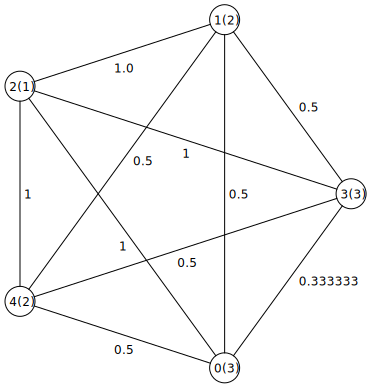
\includegraphics[scale=.6]{images/content/05_workflowTime/simpleFrameToGraph}
\caption{Erzeugung eines Graphen aus Dokumenten und den zugewiesenen Themen mittels des Algorithmus \CST}
\label{fig:simpleFrameToGraph}
\end{figure}

\subsection{Dokumentzentrierter Graph (\CDC)}
\label{subsec:cdc}

Der zweite Algorithmus erzeugt keinen vollständig verbundenen Graphen. 
Im Einzelnen werden, ähnlich wie im vorhergehenden Algorithmus \CST, die Themen der Dokumente mit einer Wahrscheinlichkeit größer als ein angegebener Schwellwert als Knoten in den Graphen eingefügt. Allerdings werden nur noch Kanten gezogen, wenn die Themen in den Dokumenten vorkommen. Da gleiche Themen oft in verschiedenen Dokumenten vorkommen, ergibt sich wieder ein zumindest schwach zusammenhängender Graph. Ein Thema, das in allen Dokumenten vorkommt, wird mit allen anderen Themen verbunden sein. Dies kann man in Abbildung \ref{fig:documentCentricFrameToGraph} sehen. Hier kommt Thema 1 in jedem Dokument vor und verbindet deshalb alle Dokumentsubgraphen miteinander. Thema 6 und 4 kommen in zwei Dokumenten vor und verbinden somit zwei Dokumente. Hier ist es jedoch möglich, dass ein Dokument nur aus Themen zusammengesetzt ist, die in keinem anderen Dokument vorkommen. So entsteht ein nicht verbundener Graph. 

\begin{figure}[ht]
\centering
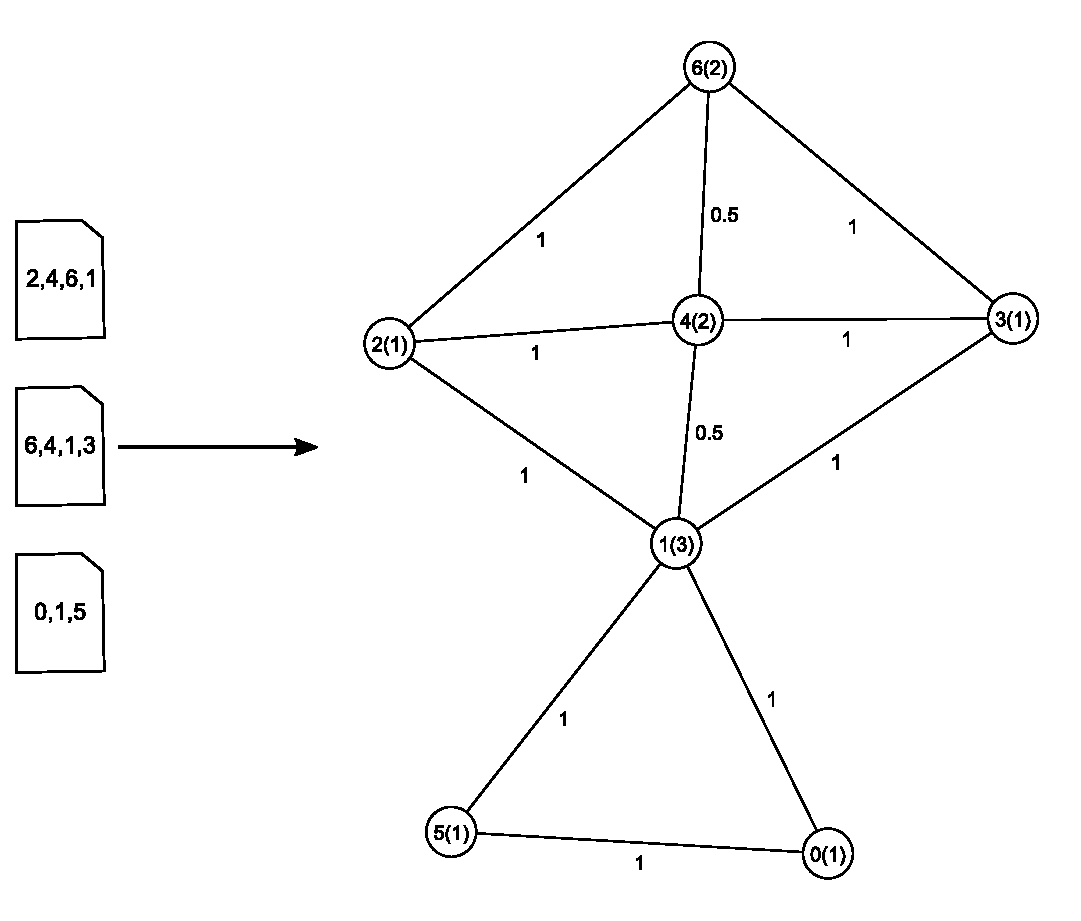
\includegraphics[scale=.6]{images/content/05_workflowTime/documentCentricFrameToGraph.eps} 
\caption{Erzeugung eines Graphen aus Dokumenten und den zugewiesenen Themen mittels des Algorithmus \CDC}
\label{fig:documentCentricFrameToGraph}
\end{figure}

Der Algorithmus zur Erstellung der Graphen funktioniert ähnlich zum vorhergehenden. Es wird für jedes Dokument ein vollständig verbundener Subgraph erstellt. Dies wird in Algorithmus \ref{lst:documentCentricFrameGraph}, in den Zeilen 3 bis 16 codiert. Dort werden auch die Themen $\docTopic_k$ als Knoten eingefügt, deren Wahrscheinlichkeit $\docTopicProb{m}{k}$ größer als der Schwellwert ist. Dann wird für jeden Knoten im Subgraphen $G_m=(V_m,E_m)$ eine Kante zu jedem anderen Knoten gezogen. Wenn eine Kante im globalen Graphen $G=(V,E)$ schon vorhanden ist, muss das Gewicht dieser Kante angepasst werden. Dazu wird analog wie in Algorithmus \ref{lst:countingSimpleTopicToGraph} erst die Anzahl der Vorkommen dieser Kante bestimmt und dann das Gewicht angepasst (siehe Zeile 8-10). Wenn der Subgraph $G_m$ erstellt wurde, werden die Knotenmengen und Kantenmengen des Subgraphen mit dem globalen Graphen vereinigt. 

\begin{algorithm}[ht]
\begin{algorithmic}[1]
\STATE $V = \emptyset, E = \emptyset$
\FORALL{$\doc_m \in \frame$}
  \STATE $V_m = \emptyset, E_m = \emptyset$
  \STATE $V_m = \left\lbrace k | \docTopicProb{m}{k} > \epsilon \right\rbrace$
  \FOR{$k \in V_m$}
    \FOR{$v \in V_m$}
      \IF{$\left\lbrace v,k \right\rbrace \in E \wedge v \neq k$}
        \STATE $oldWeight = \edgeWeight{\left\lbrace v,k \right\rbrace}$ 
        \STATE $count = \frac{1}{oldWeight}$	
	    \STATE $\edgeWeight{\left\lbrace v,k \right\rbrace} = \frac{1}{count + 1}$
      \ELSE
        \STATE $E_m = E_m \cup \left\lbrace \left\lbrace v,k \right\rbrace \right\rbrace$
        \STATE $\edgeWeight{\left\lbrace v,k \right\rbrace} = 1$
      \ENDIF
    \ENDFOR
  \ENDFOR
  \STATE $V = V \cup V_m$
  \STATE $E = E \cup E_m$
\ENDFOR 
\end{algorithmic}
\label{lst:documentCentricFrameGraph}
\caption{Dokument zentrischer Graphenalgorithmus (\CDC)}
\end{algorithm}

Hier ist es gleichfalls möglich, den Algorithmus direkt in Mengenschreibweise anzugeben. Es muss wieder festgehalten werden, wie oft ein Thema in die Knotenmenge eingefügt wurde. Die Knotenmenge ist die gleiche wie im vorhergehenden Algorithmus: Sie enthält alle Themen, deren Dokument-Wahrscheinlichkeit größer als $\epsilon$ ist. 
\[
V = \bigcup_{\doc_m \in \frame} \left\{ k | \docTopicProb{m}{k} > \epsilon\right\}
\]

Allerdings wird nicht mehr jeder Knoten mit allen anderen Knoten verbunden. Es werden nur noch die Knoten verbunden, für die gilt, dass sie im selben Dokument vorkommen und ihre Dokumentwahrscheinlichkeit größer als der geforderte Schwellwert ist. 
\[
E = \bigcup_{\doc_m \in \frame} \left\{ {i,j} | \docTopicProb{m}{i} > \epsilon \wedge \docTopicProb{m}{j} > \epsilon, i \neq j \right\}
\]

Die Kantengewichte wiederum werden analog zum vorhergehenden Algorithmus bestimmt. 
 \[
 \omega(\{i,j\}) = \frac{1}{min \{count(i),count(j)\} } 
 \]


\subsection{Graph mit Themenwahrscheinlichkeit (\TPR)}
\label{subsec:tpr}

Der nächste Algorithmus berücksichtigt die Wahrscheinlichkeit der Themen in den Dokumenten. Anhand der Wahrscheinlichkeiten werden die Gewichte der Kanten berechnet. Ansonsten wird der Graph wie in Abschnitt \ref{subsec:cdc} aufgebaut. Zuerst werden alle Themen des aktuellen Dokuments, deren Wahrscheinlichkeit größer als $\epsilon$ sind, als Knoten in den Subgraphen eingefügt. Danach werden zwischen allen Knoten des Subgraphen Kanten gezogen. Wenn die Kante im globalen Graphen noch nicht existiert, wird sie im Subgraphen hinzugefügt mit einem initialen Gewicht das dem inversen F-Wert der beiden Themenwahrscheinlichkeiten $k$ und $v$ im Dokument $m$ entspricht. Ist die Kante im globalen Graphen schon vorhanden, wird das Gewicht folgendermaßen angepasst: Das neue Gewicht berechnet sich als Produkt des alten Gewichtes mit dem inversen F-Wert der Themenwahrscheinlichkeiten der beiden Themen $k$ und $v$ im Dokument $m$.
\begin{equation}
1 - \frac{2 \cdot \docTopicProb{m}{v} \cdot \docTopicProb{m}{k}}{\docTopicProb{m}{v} + \docTopicProb{m}{k}}
\label{eq:topicProbWeightFScore}
\end{equation}
Der inverse F-Wert in Gleichung \ref{eq:topicProbWeightFScore} nähert sich für zwei hohe Wahrscheinlichkeiten $\docTopicProb{m}{v}$ und $\docTopicProb{m}{k}$ Null an und für zwei niedrige Wahrscheinlichkeiten Eins an. Das heißt, zwei Knoten mit hoher Wahrscheinlichkeit liegen näher beieinander als zwei Knoten mit niedriger Wahrscheinlichkeit. Durch die Anpassung der Gewichte wird die Distanz zweier Themenknoten, die häufiger zusammen auftreten, kleiner. Dies ist für die später berechneten Zentralitätsindizes wichtig.

\begin{algorithm}[ht]
\begin{algorithmic}[1]
\STATE $V = \emptyset, E = \emptyset$
\FORALL{$\doc_m \in \frame$}
  \STATE $V_m = \emptyset, E_m = \emptyset$
  \STATE $V_m = \left\lbrace k | \docTopicProb{m}{k} > \epsilon \right\rbrace$
  \FOR{$k \in V_m$}
    \FOR{$v \in V_m$}
      \IF{$\left\lbrace v,k \right\rbrace \in E \wedge v \neq k$}
        \STATE $\edgeWeight{\left\lbrace v,k \right\rbrace} = \edgeWeight{\left\lbrace v,k \right\rbrace} \cdot \left( 1 - \frac{2 \cdot \docTopicProb{m}{v} \cdot \docTopicProb{m}{k}}{\docTopicProb{m}{v} + \docTopicProb{m}{k}}\right)$
      \ELSE
        \STATE $E_m = E_m \cup \left\lbrace \left\lbrace v,k \right\rbrace \right\rbrace$
        \STATE $\edgeWeight{\left\lbrace v,k \right\rbrace} = 1 - \frac{2 \cdot \docTopicProb{m}{v} \cdot \docTopicProb{m}{k}}{\docTopicProb{m}{v} + \docTopicProb{m}{k}}$
      \ENDIF
    \ENDFOR
  \ENDFOR
  \STATE $V = V \cup V_m$
  \STATE $E = E \cup E_m$
\ENDFOR 
\end{algorithmic}
\label{lst:topicProbFrameGraph}
\caption{Graph mit Themenwahrscheinlichkeit (\TPR)}
\end{algorithm}

Die Definition des Graphen in Mengenschreibweise ist wie folgt. Die Knoten des Graphen sind wieder diejenigen Themen deren Wahrscheinlichkeit in einem Dokument des Frames größer als $\epsilon$ ist.
\[
V = \bigcup_{\doc \in \frame} \left\{ k | \docTopicProb{m}{k} > \epsilon\right\}
\]

Die Kanten werden zwischen Themenknoten gezogen, die in demselben Dokument vorkommen, analog zum vorhergehenden Algorithmus.
\[
E = \bigcup_{\doc_m \in \frame} \left\{ {i,j} | \docTopicProb{m}{i} > \epsilon \wedge \docTopicProb{m}{i} > \epsilon, i \neq j \right\}
\]

Das Gewicht einer Kante von $i$ nach $j$ berechnet sich als das Produkt des inversen F-Wertes der Wahrscheinlichkeit des Themas $i$ und $j$ in allen Dokumenten, in denen die Themen $i$ und $j$ zusammen auftreten. Dies entspricht dem mehrmaligen Einfügen einer Kante, wie es im Algorithmus aufgeführt wird.
\[
\omega(\{i,j\}) = \prod_{m : \docTopicProb{m}{i} > \epsilon \wedge \docTopicProb{m}{j} > \epsilon} 1 -
\frac{2 \cdot \docTopicProb{m}{i} \cdot \docTopicProb{m}{j}}{\docTopicProb{m}{i} + \docTopicProb{m}{j}}
\]


\section{Zentralitäten}

Auf die so erstellten Graphen werden nun die in Kapitel \ref{chap:basics} vorgestellten Zentralitätsindizes angewendet. Für jeden Zeitabschnitt gibt es einen Graphen, dessen Knoten die vorkommenden Themen repräsentieren und der die Wahrscheinlichkeit der Themen in der Struktur des Graphen enthält. Im Falle der beiden Algorithmen \CST$\;$und \CDC$\;$ist die Wahrscheinlichkeit implizit enthalten, im Falle des Algorithmus \TPR$\;$explizit. Dennoch kann mit Hilfe der Zentralitätsindizes die Wichtigkeit der Themen bestimmt werden.

\subsection{Normalisierung}
Zur besseren Vergleichbarkeit der Ergebnisse der unterschiedlichen Zentralitäten werden die Verläufe normalisiert. Die Normalisierung der Zentralitätsindizes kann einerseits pro Graph vorgenommen werden oder über alle betrachteten Frames. 

Bei der Normalisierung pro Graph werden die Zentralitätsindizes der Knoten auf den Wertebereich $[0,1]$ abgebildet. Für jeden Graphen werden die Zentralitätsindizes anhand der $L^\infty$-Norm normalisiert, indem die einzelnen Zentralitätswerte der Knoten durch den maximalen Zentralitätswert im Graphen geteilt werden. Die normalisierte Zentralität $\centrality{nX}$ für einen Knoten $v$ im Graphen $G=(V,E)$ mit Zentralität $\centrality{X}(v)$ ist
\begin{equation*}
\centrality{nX}(v) = \frac{\centrality{X}(v)}{\max_{u \in V}\left\lbrace\centrality{X}(u)\right\rbrace}\text{.}
\end{equation*}
So erhält man für jeden Graphen Zentralitätswerte zwischen Null und Eins. Leider lassen sich damit verschiedene Graphen nicht ohne weiteres vergleichen \citep{Brandes2005}, was direkte Auswirkungen auf die Vergleichbarkeit der prominenten Themen in den aufeinanderfolgenden Frames hat.

Es wird deshalb eine Normalisierung vorgeschlagen, die nicht die einzelnen Graphen normalisiert, sondern über alle Frames normalisiert. Hierzu wird auch die $L^\infty$-Norm verwendet jedoch, wird nicht mehr der Maximalwert eines einzelnen Graphen benutzt, sondern der Maximalwert aller Graphen bzw. Frames. 

Sei $G_{\frame_i}=(V_{\frame_i},E_{\frame_i})$ der korrespondierende Graph zu Frame $\frame_i$. Dann werden die Zentralitätswerte folgendermaßen normalisiert:
\begin{equation*}
\centrality{nX}(v) = \frac{\centrality{X}(v)}{\max_{u \in V_{\frame_i}\ \forall \frame_i \in \corpus }\left\lbrace\centrality{X}(u)\right\rbrace}\text{.}
\end{equation*}
So wird die Vergleichbarkeit der unterschiedlichen Graphen und der verschiedenen Zentralitätsindizes gewährleistet, da jeder Knoten relativ zu allen Graphen bewertet wurde. In der späteren Online-Applikation ist eine Normalisierung nicht mehr möglich, da man im Voraus das Maximum nicht bestimmen kann. Da die Normalisierung aber nur zur Vergleichbarkeit der Zentralitätsindizes benutzt wird, sollten die absoluten Werte ausreichend sein.

\subsection{Nicht verbundene Graphen}
Bei den letzten beiden, in Abschnitt \ref{sec:topic2graph} beschriebenen Algorithmen kann es vorkommen, dass diese einen Graph erzeugen, der nicht verbunden ist. Wie schon in den Grundlagen dargelegt wurde, sind einige Zentralitätsindizes nicht auf unzusammenhängenden Graphen definiert. 

Ein Ansatz dieses Problem zu handhaben, besteht darin die Zentralitätsindizes für jede Zusammenhangskomponente einzeln zu berechnen und die Werte dann mit der Größe der Komponente zu gewichten. Dies funktioniert, solange der Zentralitätsindex sich proportional zur Größe des Graphen verhält \citep{Brandes2005}. Die Closeness- und Eccentricity-Zentralität verhalten sich jedoch nicht proportional zur Größe des Graphen \citep{Poulin2000}. Somit werden die Ergebnisse dieser Zentralitäten für unzusammenhängende Graphen unbrauchbar. Gleichzeitig haben Poulin, Boily und Mâsse \citep{Poulin2000} einen neuen Zentralitätsindex entwickelt, der auch für unzusammenhängende Graphen funktioniert. Da der Fall, dass ein nicht zusammenhängender Graph erzeugt wird, jedoch selten auftritt und durch geeignete Wahl der Framegröße und der Frameüberlappung umgangen werden kann, wurde dieser Zentralitätsindex hier nicht implementiert. 

Es wird jedoch folgende Heuristik verwendet, um unzusammenhängende Graphen bewerten zu können. Es wird generell die Zusammenhangskomponente mit der größten Anzahl an Knoten bewertet. Zusammenhangskomponenten, die um bis zu 20\% von der Maximalgröße abweichen, werden ebenfalls bewertet. In allen anderen Zusammenhangskomponenten werden die Zentralitätswerte der Knoten auf Null gesetzt. So entdeckt man einen Themenbruch innerhalb eines Frames, wenn die Themen in ungefähr gleich vielen Dokumenten erwähnt sind. 
\section{Visualisierung}
\begin{figure}[ht]
\centering
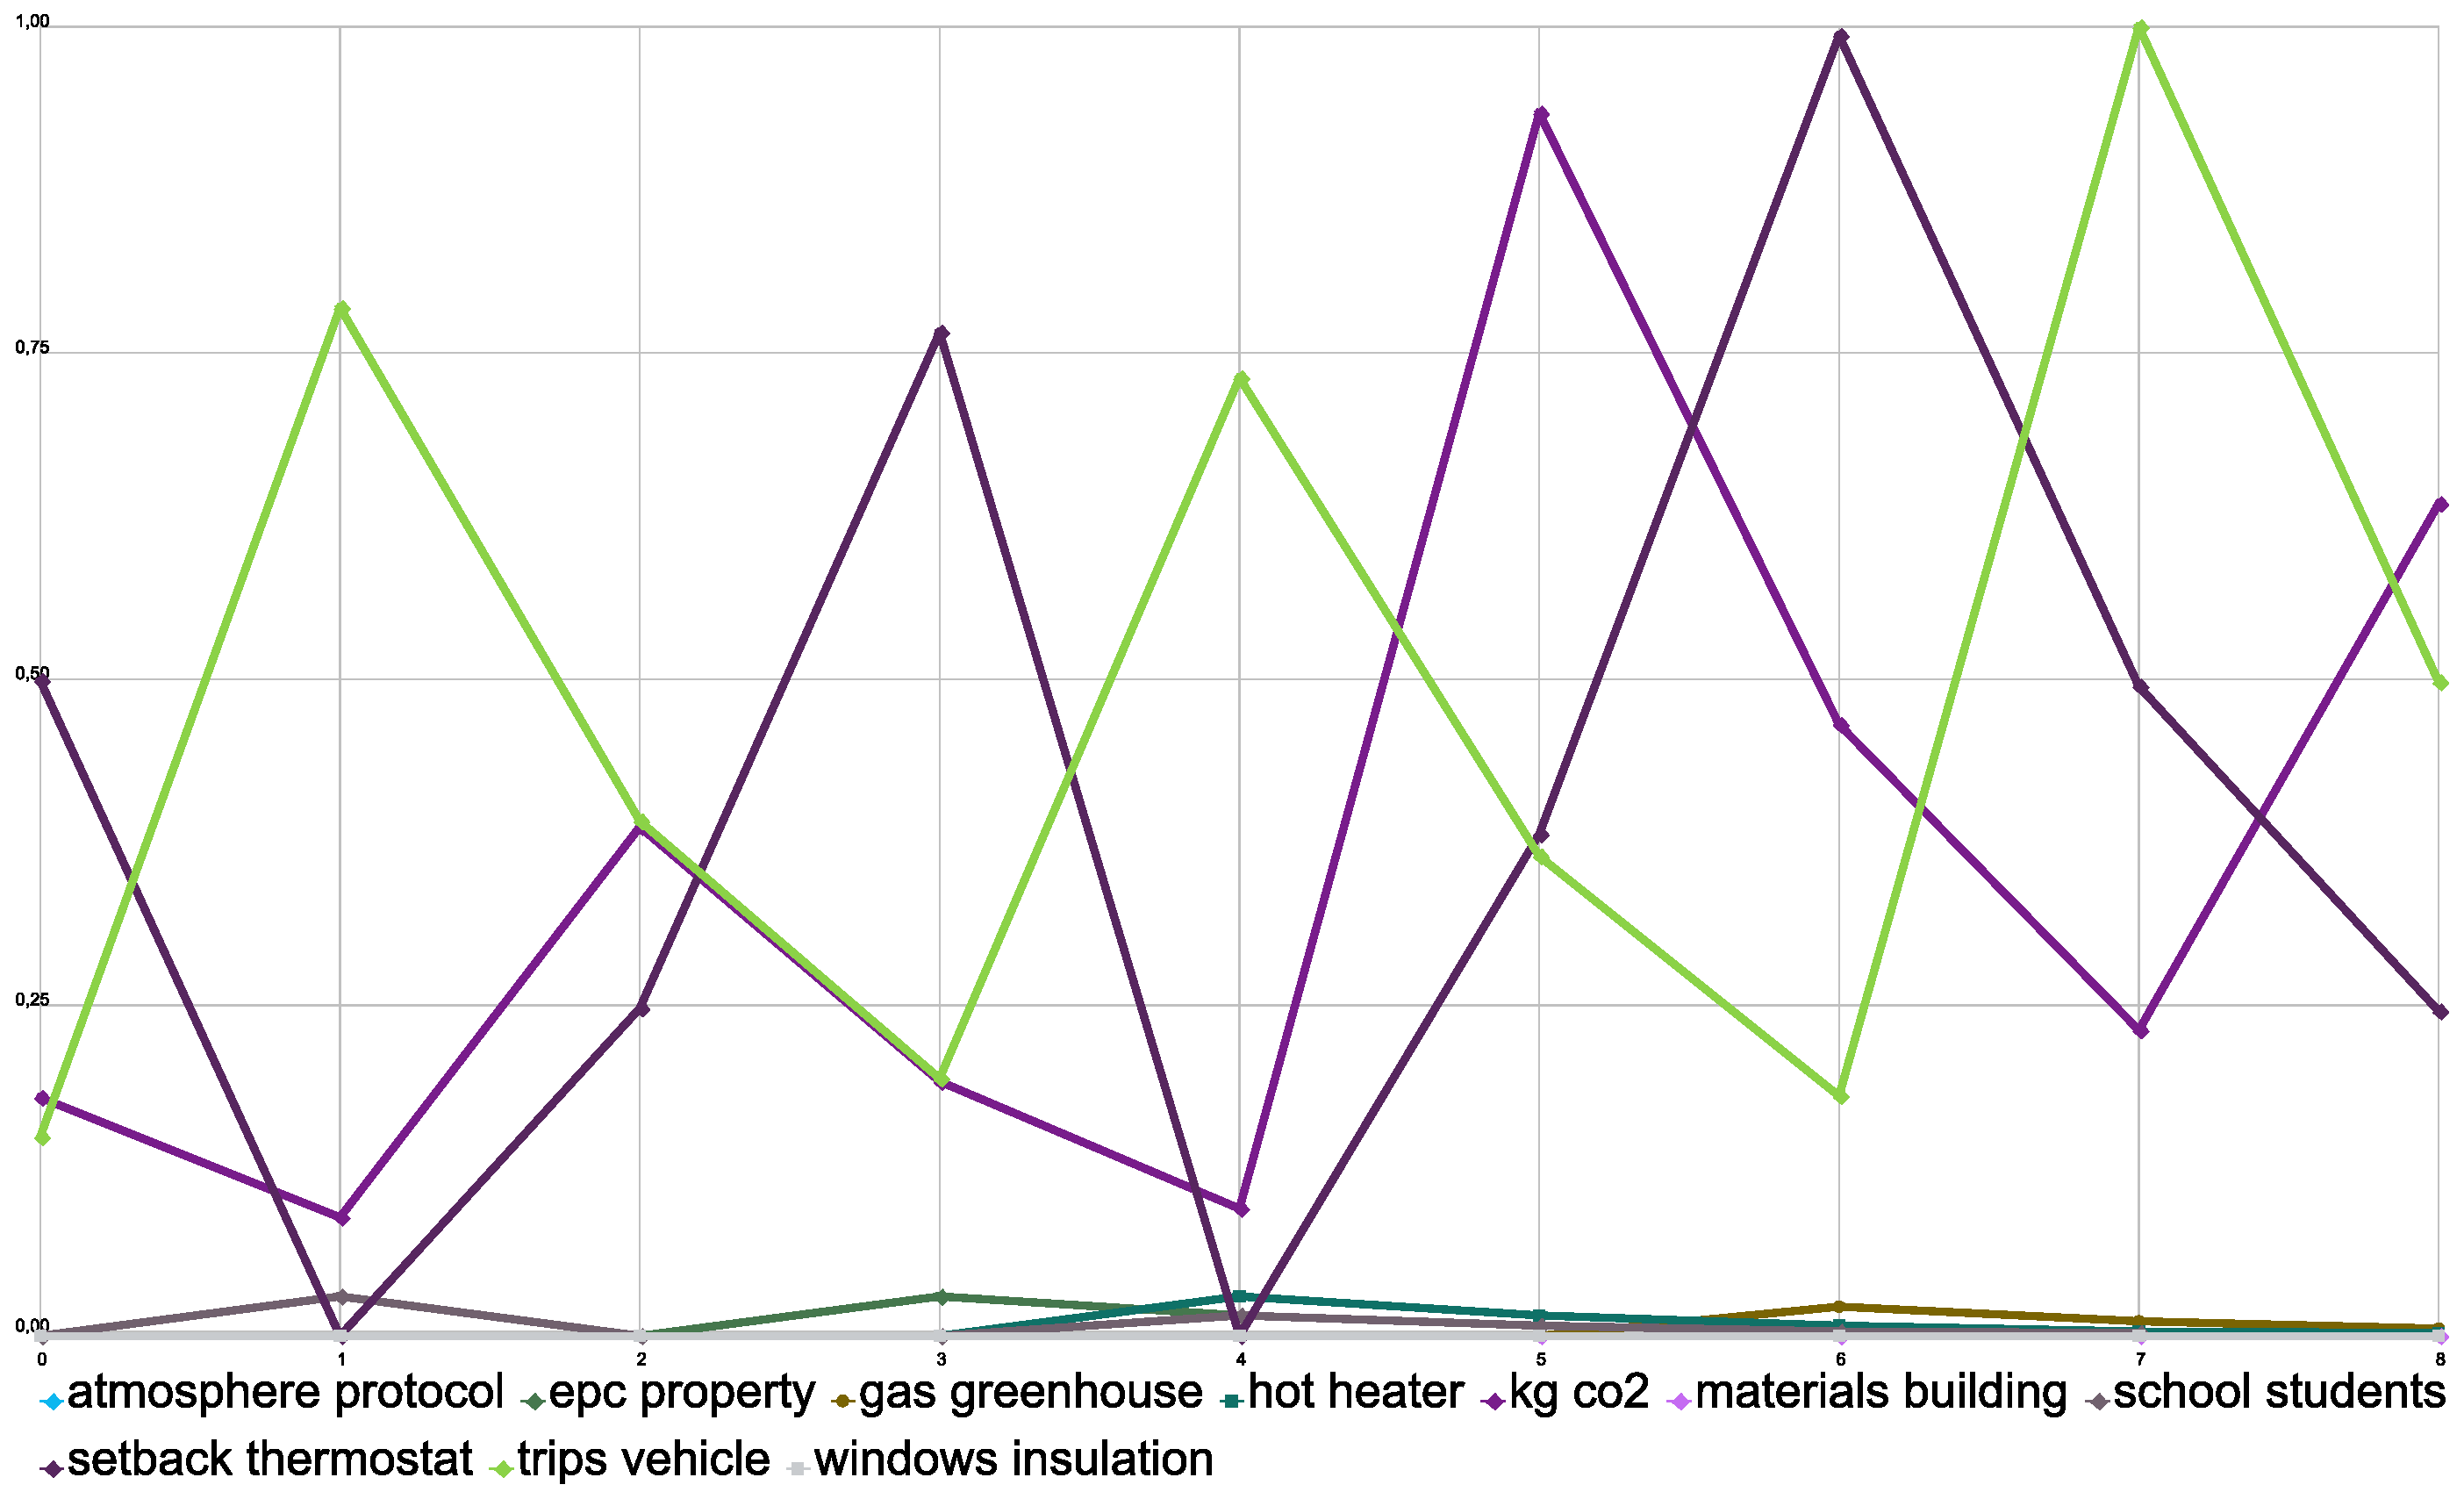
\includegraphics[width=\textwidth, height=0.5\textheight]{images/content/05_workflowTime/allInOne.eps} 
\caption{Alle Themenverläufe in einem Diagramm. Auf der X-Achse ist die Framezahl aufgetragen, auf der Y-Achse die normalisierte Zentralität}
\label{fig:allInOne}
\end{figure}

Für die Visualisierung der Themenverläufe wurde eine eigene Komponente entwickelt, die die Verläufe darstellt. Es wurden zwei Arten der Visualisierung implementiert. In der ersten Variante werden die Themenverläufe als Liniendiagramm in dasselbe Koordinatensystem eingezeichnet. Auf der X-Achse wird die laufende Framenummer abgetragen und auf der Y-Achse die normalisierte Zentralität. Jedes Thema wird durch eine eigene Linie repräsentiert. Welche Linie welches Thema repräsentiert wird als Beschriftung unterhalb des Diagramms eingeblendet (siehe Abbildung \ref{fig:allInOne}). 

\begin{figure}[ht]
\centering
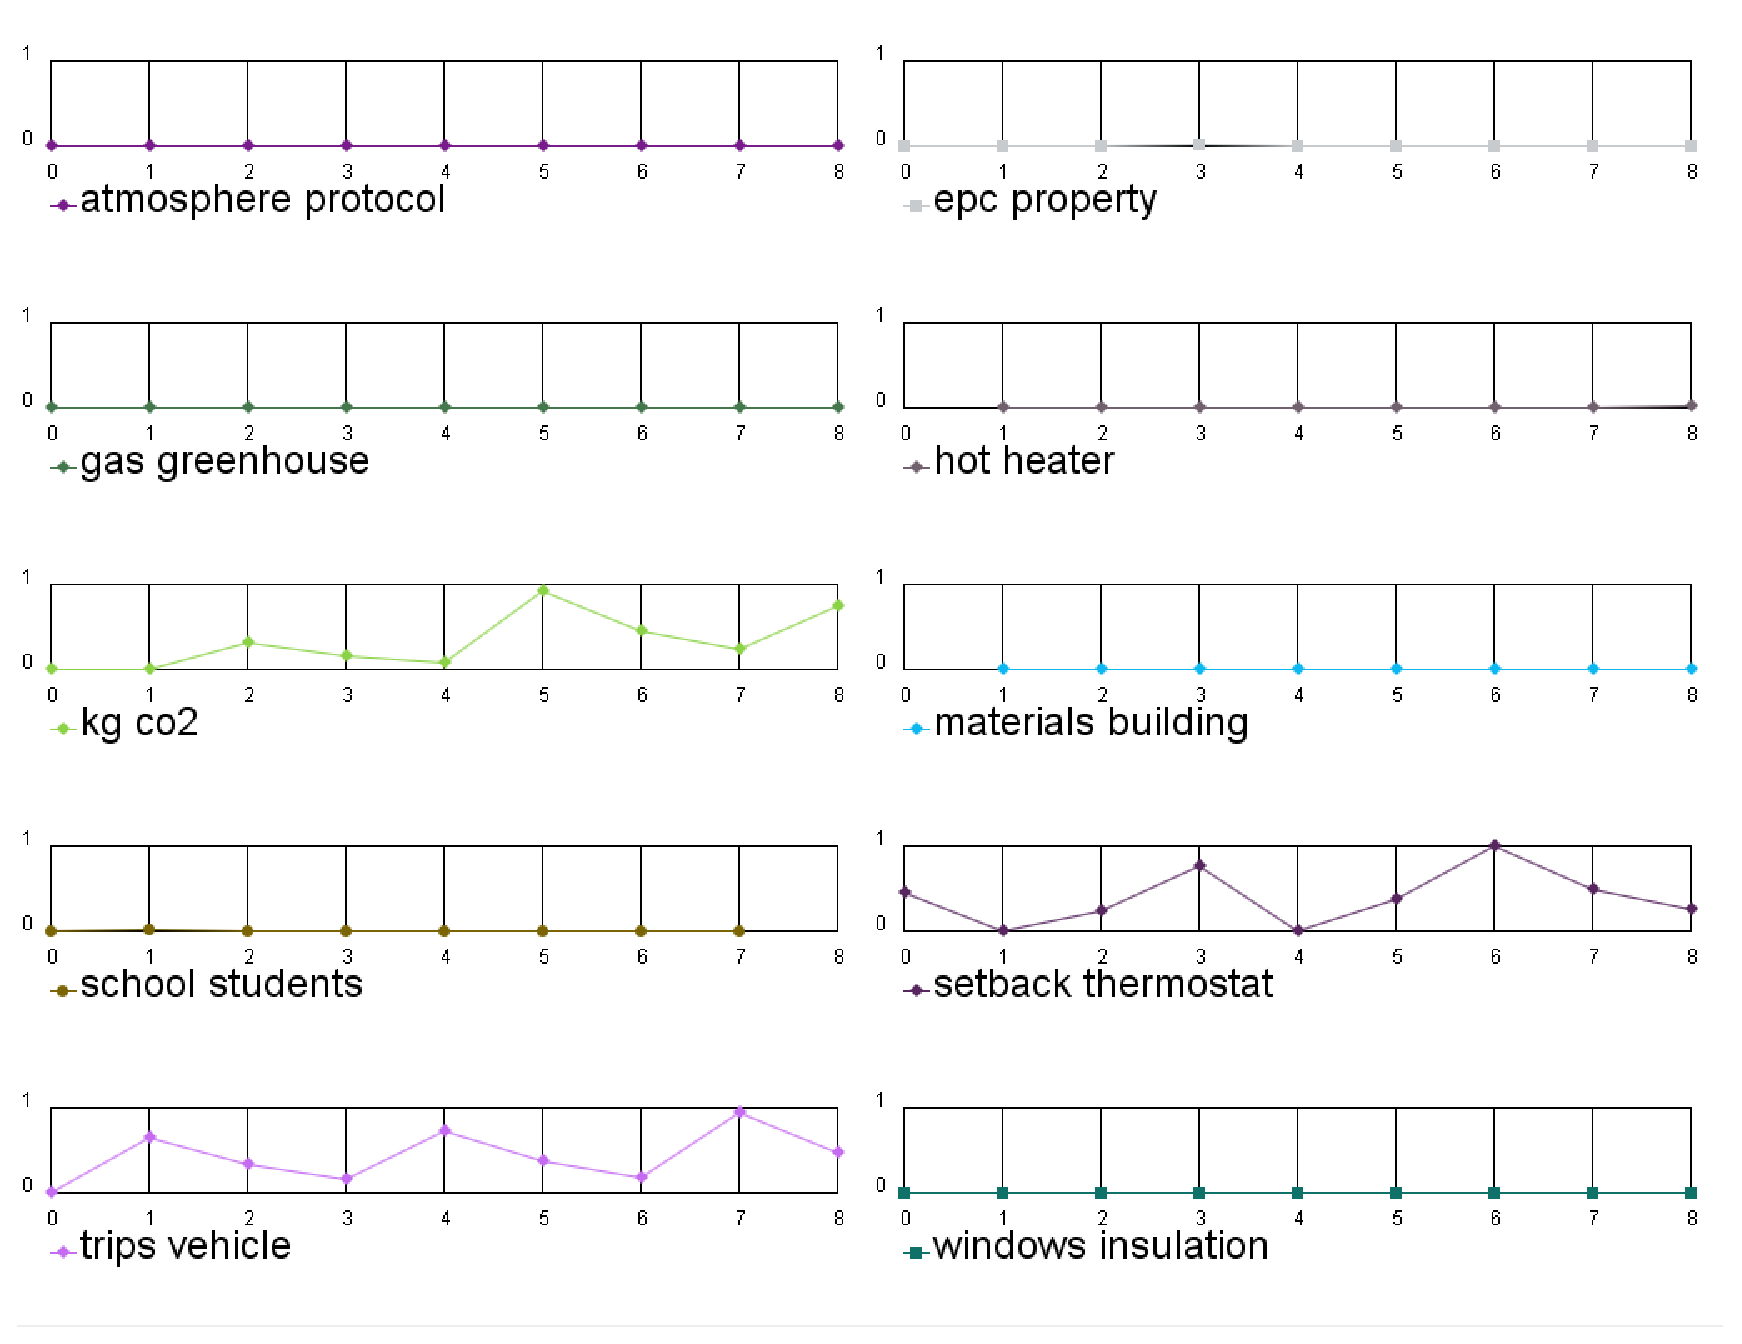
\includegraphics[width=\textwidth]{images/content/05_workflowTime/separatedViews.eps} 
\caption{Jeder Themenverlauf in einem eigenen Diagramm. Auf der X-Achse ist die Framezahl aufgetragen, auf der Y-Achse die normalisierte Zentralität}
\label{fig:separatedViews}
\end{figure}

Bei dieser Art der Visualisierung kann das Problem auftreten, dass die Prominenz der Themen nicht mehr differenziert werden kann, wenn viele Themen einen ähnlichen Verlauf haben, bzw. einen Verlauf auftritt, der viele andere Verläufe schneidet. Andererseits können bei Verläufen, in denen nicht viele Themen eine hohe Prominenz aufweisen, mit einem Blick die wichtigen Themen abgelesen werden und das Verhältnis zu den anderen Themen bestimmt werden.

In der zweiten Variante zeichnet man die Themenverläufe jeweils in ein eigenes Diagramm ein (siehe Abbildung \ref{fig:separatedViews}). Diese Diagramme werden dann in einer Matrix angeordnet. Diese Art der Visualisierung hat den Vorteil, dass man besser differenzieren kann, welche Themen wichtig sind. Jedoch ist die relative Zentralität eines Themas im Verhältnis zu anderen Themen schwieriger zu erkennen.

\section{Methoden der Evaluation}
\label{sec:centralityEvaluation}
Die Validierung der Themenverläufe stellt eine Schwierigkeit dieser Diplomarbeit dar. Bisher haben sich wenige Arbeiten mit der Evaluation von Themenverläufen beschäftigt. Es gibt dementsprechend wenige publizierte Ansätze zur Validation. In \citep{onlineLDA2} sollen Thementrends ähnlich zu dieser Diplomarbeit erkannt werden. Um den Algorithmus zu testen, werden Textsequenzen untersucht. Die Evaluation erfolgt nun durch zurückhalten von Dokumenten zu speziellen Themen, die ab einem vorher definierten Zeitpunkt in die Sequenz eingefügt werden. Entdeckt der Algorithmus diese Themen an dem definierten Zeitpunkt, wird dies als Erfolg gewertet. 

Diese Art der Evaluation wird in der Diplomarbeit auch verwendet. Es werden jedoch nicht reale Dokumente aus einem Testkorpus benutzt und Dokumente zurückgehalten, sondern die Dokumente werden künstlich erzeugt. Es wird der generative Prozess des LDA-Modells genutzt, um Dokumente zu erzeugen, die definierte Themen mit einer festen Wahrscheinlichkeit enthalten. Erzeugt man mehrere Dokumente auf diese Weise, können Testdaten erzeugt werden, die vorher definierte Themenverläufe aufweisen. Diese Testdaten werden dann dazu benutzt zu evaluieren, ob erstens die Verläufe tatsächlich entdeckt werden und wie gut sie durch den verwendeten Zentralitätsindex wiedergegeben werden. Dazu wird numerisch bestimmt, wie gut der Themenverlauf erfasst wird; einerseits von einer analytischen und andererseits von einer kognitiven Perspektive.

\subsection{Synthetische Verläufe}

Für jedes Themenmodell werden jeweils synthetische Textsequenzen erzeugt, anhand derer fest definierte Themenverläufe erzeugt werden. Es werden verschiedene Themenverläufe mit jeweils anderen Wahrscheinlichkeiten der Themen in den Dokumenten erzeugt. Insgesamt werden pro Themenmodell fünf Verläufe generiert, die sich in der Anzahl der Dokumente, der festgelegten Themen und deren Wahrscheinlichkeit unterscheiden. 

\begin{labeling}[:]{3TSw 0.2}
\item[3TSw 0.2] Eine Textsequenzen bestehend aus 120 Dokumenten. Jedes Dokument enthält drei Themen. Jeweils ein Thema und dessen Wahrscheinlichkeit ist vorher festgelegt. Die restlichen beiden Themen und deren Wahrscheinlichkeit werden zufällig ausgewählt. Es werden jeweils zehn Dokumente mit dem gleichen festgehaltenen Thema erzeugt. Die Wahrscheinlichkeit des Themas in den Dokumenten wird auf $0,2$ gesetzt. Nach 30 Dokumenten wird wieder das Thema der ersten zehn Dokumente gewählt. Es wird erwartet, dass bei einer Framegröße von zehn eine Sägezahnkurve auftritt, in der sich jeweils drei Themen abwechseln.   

\item[3TSw 0.8] Eine Textsequenzen wie in erstens, nur dass die Wahrscheinlichkeit des festgehaltenen Themas auf $0,8$ gesetzt wird. Auch hier wird wieder eine Säge"-zahnkurve erwartet jedoch mit anderen Werten der Zentralitätsindizes.
 
\item[CT 0.2] Eine Textsequenzen aus 100 Dokumenten die jeweils ein Thema festgelegt haben und zwei Themen zufällig gewählt. Die Wahrscheinlichkeit des festen Themas wurde auf $0,2$ gesetzt. Erwartet wird, dass das festgelegte Thema als prominentestes Thema auftritt und alle anderen Themen dominiert, da das Thema häufig zusammen mit anderen Themen auftritt.

\item[CT 0.8] Die Gleiche Textsequenzen wie in drittens nur das die Wahrscheinlichkeit auf $0,8$ gesetzt wurde.

\item[3TS] Eine Textsequenzen von 100 Dokumenten mit drei Themen die gleichzeitig prominent sind. Die Wahrscheinlichkeit wurde für alle Themen auf $0,2$ gesetzt. Zusätzlich wurden zufällig drei Themen ausgewählt, auf die   Restwahrscheinlichkeit von $0,4$ zufällig aufgeteilt wurde.
\end{labeling}

Da die wichtigen Themen in den Verläufen bekannt sind, kann numerisch ermittelt werden, wie gut diese vom System erkannt werden. Um dies zu evaluieren, wird ein dem Signal-Rausch-Verhältnis ($SRV$) verwandtes Maß \TODO{cite} benutzt, welches die Verläufe der relevanten Themen als Signal auffasst und die Zentralitätswerte als Signalstärke. Das Rauschen wird als der Mittelwert aller Themenverläufe aufgefasst. Betrachtet man nur die nicht relevanten Verläufe als Rauschen, unterscheiden sich diese oft nicht signifikant vom Mittelwert. Sie werden somit als relevant klassifiziert, obwohl sie im voraus nicht als solche definiert wurden. 

Ein Verlauf stellt für eine Thema die ermittelten Zentralitätswerte über die Zeit dar. Dementsprechend kann ein Verlauf eines Themas als Vektor $\vec{v}$ aufgefasst werden. Die Komponenten stellen den Zentralitätswert zu einem bestimmten Zeitpunkt dar. So ist $v_i$ der Zentralitätswert des Verlaufs zum Zeitpunkt $i$. Die Mittelwerte aller aller Verläufe werden mit $\vec{v_m}$ bezeichnet. Das Signal-Rausch-Verhältnis der einzelnen Werte ist definiert als
\[
SRV=10 \cdot \log_{10}\left({\frac{v_i}{v_{m_{i}}}}\right)
\]
und bewegt sich in diesem speziellen Anwendungsfall im Wertebereich $[-10,\ldots,10]$.

Wenn für einen Wert eines relevanten Verlaufs das $SRV$ größer als ein fester Wert $t$ ist, wird dieser Wert als richtig positiver Fall angenommen. Ist der Wert kleiner als $t$ wird er als falsch positiv angenommen. Für nicht relevante Verläufe wird auch das $SRV$ bestimmt. Ein $SRV$-Wert der größer als $t$ ist, wird als falsch positiv klassifiziert und ein Wert der kleiner als $t$ ist, als richtig negativ. Zählt man die einzelnen Auftreten von richtig positiv, falsch positiv usw. kann man die Trefferquote \[R = \frac{\text{richtig positiv}}{\text{richtig positiv} + \text{falsch negativ}}\] und die Genauigkeit \[P = \frac{\text{richtig positiv}}{\text{richtig positiv} + \text{falsch positiv}}\] bestimmen. Aus Trefferquote und Genauigkeit kann dann ein Wert \[F=\frac{2 \cdot P \cdot R}{P+R} \] berechnet werden, der angibt wie gut ein Verlauf erkannt wurde.

In den ersten Versuchen die Themenverläufe numerisch zu bewerten, wurde ein konstanter Schwellwert benutzt, um die richtig positiven und falsch positiven Fälle zu ermitteln. Wenn der Zentralitätswert eines relevanten Verlaufes über dem Schwellwert lag wurde er als richtig positiv gewertet und wenn der Zentralitätswert eines nicht relevanten Verlauf über dem Schwellwert lag, wurde er als falsch positiv klassifiziert. Es gab allerdings Konfigurationen der Themenverläufe, in denen die nicht relevanten Verläufe einen hohen Zentralitätswert aufwiesen, die relevanten Verläufe aber klar unterschieden werden konnten. Eine solche Konfiguration ist in Abbildung \ref{fig:allInOne} dargestellt. Hier ist im sechsten Frame das Thema \textit{kg co2} das relevante und die beiden anderen Themen irrelevant. Sie würden aber als falsch positiv bewertet, obwohl sich das Thema \textit{kg co2} klar von den beiden anderen Themen abhebt. Mit dem konstanten Schwellwert wurden somit die Bewertung schlechter, obwohl die die relevanten Verläufe klar als solche erkannt werden konnten. 

Es wurde deshalb das $SRV$ verwendet, um eine adaptive Methode zur Bewertung zu haben. Mit dem $SRV$ werden solche Konfigurationen der Verläufe richtig bewertet, da es hier auf das Verhältnis von relevantem zu nicht relevantem Verlauf ankommt. Trotz der hohen Zentralitätswerte der nicht relevanten Verläufe ist die Bewertung hoch, da das Verhältnis zwischen relevantem Themenverlauf und nicht relevantem Themenverlauf hoch genug ist, um diese voneinander zu unterscheiden.
\section{Zusammenfassung}
In diesem Kapitel wurde dargelegt, wie die Anwendungsphase der entwickelten Methode funktioniert. Es wurden die einzelnen Teilschritte erläutert; insbesondere wie aus Texten ein Verlauf von Themen generiert wird, wie die Textsequenzen in Zeitabschnitte aufgeteilt werden, wie die Themen für die Dokumente in den Zeitabschnitten ermittelt werden, wie daraus wiederum Graphen aufgebaut werden und wie die Zentralitätsindizes auf diese Graphen angewendet werden und somit die Themenverläufe ermittelt werden. Zusätzlich wurde erläutert, wie die Themenverläufe visualisiert werden können und wie sie validiert werden können. Die Ergebnisse des in diesem Kapitel vorgestellten Algorithmus werden im nächsten Kapitel präsentiert. Anhand der Validierungskriterien wird ermittelt, welche Zentralitätsindizes geeignet sind, die Themenverläufe zu erfassen.

